\documentclass{article}

\usepackage[utf8]{inputenc}
\usepackage[T1]{fontenc}
% \usepackage[slovene]{babel}
\usepackage{lmodern}
\usepackage{hyperref}
\usepackage[ruled,vlined]{algorithm2e}
\usepackage{amsmath}

\newcommand*\mean[1]{\bar{#1}}
\newcommand*\est[1]{\hat{#1}}

\usepackage{Sweave}
\begin{document}
\input{orchard-concordance}

\title{Will we win the Orchard game?}
\author{Sara Pia Marinček}
\date{}

\maketitle

\section{The \emph{Orchard} game}
HABA's \emph{Orchard} game is a cooperative children's game. There are four fruit trees: an apple tree with 10 apples, a pear tree with 10 pears, a cherry tree with 10 pairs of cherries and a plum tree with 10 plums. The players try to pick the fruit from the trees before the raven enters the orchard. The players throw the die.
\begin{itemize}
\item If green (apple), yellow (pear), red (pair of cherries) or blue (plum) colour appears on the die, the player picks a fruit of the corresponding color and puts it into the basket. If there are no more fruits left on the tree nothing happens.
\item If the basket appears on the die, the player can pick any two fruits and place them into the basket.
\item If the raven appears on the die, the raven makes one step towards the orchard.
\end{itemize}
If the players succeed in harvesting all the fruit before the raven has reached the orchard, they win the game. If the raven makes 10 steps before all the fruits have been picked, the players lose.

In another variation of the game, \emph{My First Orchard} game, there are 4 fruits of each type, and the raven needs to take 6 steps to reach the orchard.

\subsection{Playing strategies}
When the basket appears on the die, the player can either pick fruits at random or take the strategy of choosing the fruit of the type with the most pieces left. For the latter option, we intuitively expect better chances of winning: if we decrease the number of available fruit types, then the odds of the next die roll resulting in an unfavourable color (for which there are no more fruits left on the trees) increase.

What is the probability of winning the game?

\subsection{Our methods}
To assess the probability of winning the game in each of the four scenarios (two variations of the game, two playing strategies), we will first perform a simulation (make the computer play many many games for us). Then, we will present an analytic approach for computing the probability of the game ending in any specific (final) state (and make the computer numerically evaluate the probability of winning). The code in Python is available on \href{https://github.com/sarastra/Orchard}{GitHub}\footnote{https://github.com/sarastra/Orchard}.

\section{Simulation}
\label{sim}

The computer algorithm that plays the game is straightforward. We characterize a game state as a list of remaining raven steps, apples, pears, pairs of cherries and plums. We start in the initial state with the maximum number of raven steps (10 for the \emph{Orchard} and 6 for the \emph{My First Orchard} variation), and all the fruits yet to be picked (10 fruits of each type for the \emph{Orchard} and 4 for the \emph{My First Orchard} variation). Then we roll the die until we reach the final state, with either all the fruits harvested (in which case the players win) or no raven steps left (in which case the players lose). See Algorithm \ref{rolling the die}.

\begin{algorithm}[h]
\SetAlgoLined
\While{the state is not final}{
  draw an integer \(n\) from 0 to 5 at random\;
  \uIf{\(n = 0\)}{
    decrease the number of raven steps by 1\;
   }
  \uElseIf{\(0 < n < 5\)}{
    \tcc{1 = apple, 2 = pear, 3 = cherries, 4 = plum}
    \eIf{at least one fruit of the drawn type is left}{
      pick one fruit of the drawn type\;
    }{
      do nothing\;
    }
  }
  \Else(\tcc*[h]{5 = basket}){
    \eIf{you play smart}{
      pick the fruit of the type with the most pieces left\;
    }{
      pick a fruit at random\;
    }
  }
}
\caption{Rolling the die in the First Orchard variation}
\label{rolling the die}
\end{algorithm}

When the loop ends, we check if there are more than 0 raven steps left, in which case we won. For the \emph{Orchard} variation we have to be a little careful when the basket appears on the die: after we pick the first fruit, we have to make sure that the resulting state is not final.

The outcome of a single game \(X_i\) is a Bernoulli random variable which takes the value 1 (players win) with probability \(p\) and the value 0 (players lose) with probability \(q = 1 - p\), thus \(E(X_i) = p\) and \(\mathrm{Var}(X_i) = p(1-p)\). We would like to estimate \(p\) by simulating many many games (with independent and identically distributed outcomes). According to the \emph{law of large numbers}, the sample mean will converge in probability to the population mean,
\[
  \lim_{n \to \infty} P \left(|\mean{X}_n - p| \geq \epsilon\right) = p \, ; \quad       \mean{X}_n = \frac{1}{n} \sum_{i=1}^n X_i.
\]
According to the central limit theorem, the sample mean will converge in distribution to the normal distribution,
\begin{equation}
\label{clt}
  \lim_{n \to \infty} P \left(\frac{\mean{X}_n-p}{\sqrt{p(1-p)/n}} \leq x \right) = \Phi(x) \, ,
\end{equation}
where \(\Phi(x)\) is the standard normal cumulative distribution function. If we want to provide a confidence interval for \(p\) from a single sample it comes in handy that Eq.~(\ref{clt}) also holds if we replace the standard error in the denominator with its unbiased estimate \(\est{p}(1-\est{p})/(n-1)\). It follows that for large enough \(n\) the \(100(1-\alpha)\%\) confidence interval for the parameter \(p\) will be
\begin{equation}
\label{ci}
  \est{p} \pm z_{\alpha/2} \sqrt{\frac{\est{p}(1-\est{p})}{n-1}} \, , \quad \Phi(z_{\alpha/2}) = 1 - \frac{\alpha}{2}.
\end{equation}
Depending on how wide we can afford our confidence interval to be, we can assess the (approximate) number of iterations \(n\) needed not to exceed the maximum desired width \(w_{max}\) from Eq.~(\ref{ci}):
\[
  n-1 \geq \frac{4z_{\alpha/2}^2\est{p}(1-\est{p})}{w_{max}^2} \geq \frac{z_{\alpha/2}^2}{w_{max}^2}.
\]

If we take \(n = \) 10000, we expect that the 95\% confidence interval will be at most 0.02 wide, whereas for \(n = \) 1e+08 we expect it should not be wider than 2e-04.

\subsection{Results}


Fig.~\ref{hist} shows the results for 10000 simulations of \(n = \) 10000 games, and black lines represent the (appropriately scaled) normal densities, computed as described in Sec.~\ref{analytic}, to which the distributions of sample proportions converge. We see that for both variations of the game the increase in probability of winning when playing smart is large enough that we can conclude with great confidence that picking the fruit of the type with the most pieces left does indeed make a difference.

\begin{figure}[h]
  \begin{center}
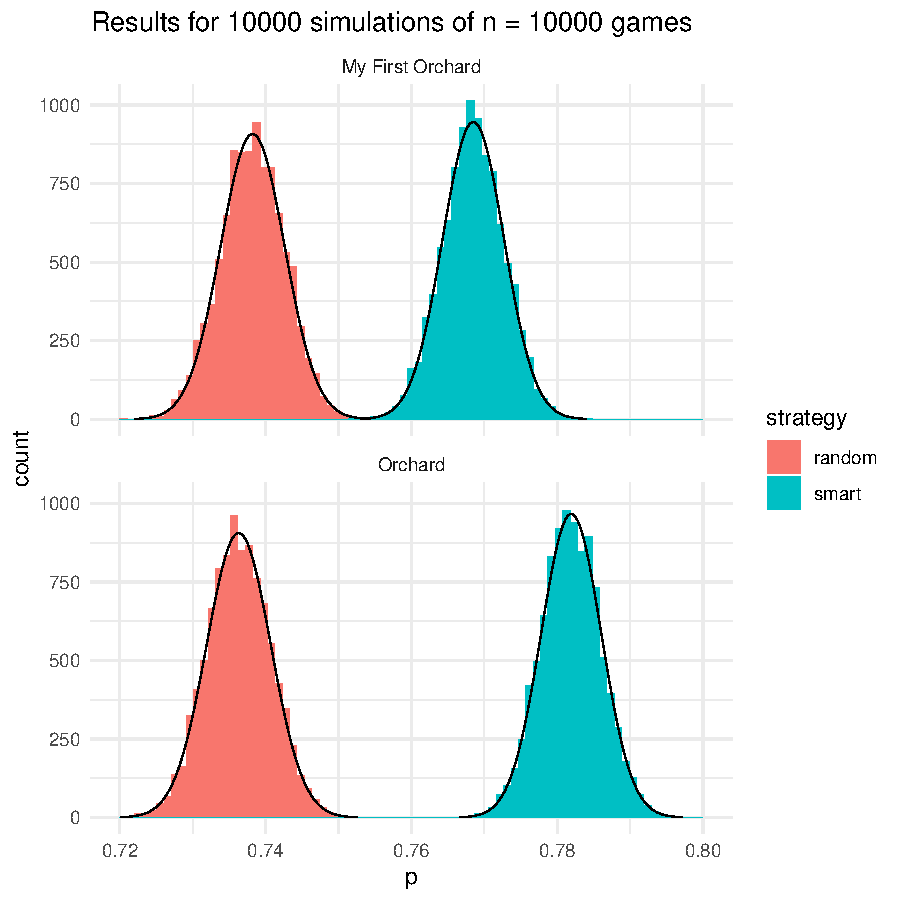
\includegraphics{orchard-003}
    \caption{Histograms showing the results of 10000 simulations of \(n = \) 10000 games. Black lines represent the (appropriately scaled) normal densities, computed as described in Sec.~\ref{analytic}, to which the distributions of sample proportions converge.}
    \label{hist}
  \end{center}
\end{figure}

Table~\ref{table} gives the results (estimated probability of winning, estimated standard error and estimated 99\% confidence interval) of a simulation of \(n = \) 1e+08 games (combining the results from all the 10000 simulations of 10000 games, the results of which are shown in Fig.~\ref{hist}), for both variations of the game and both playing strategies.

% latex table generated in R 4.0.3 by xtable 1.8-4 package
% Mon Oct 26 13:37:10 2020
\begin{table}[h]
\centering
\begin{tabular}{l|ccc}
 simulation & p & SE & 99\% CI \\ 
  \hline
My First Orchard, random & 0.73821 & 0.00004 & [0.73809, 0.73832] \\ 
  My First Orchard, smart & 0.76848 & 0.00004 & [0.76837, 0.76859] \\ 
  Orchard, random & 0.73635 & 0.00004 & [0.73623, 0.73646] \\ 
  Orchard, smart & 0.78188 & 0.00004 & [0.78177, 0.78198] \\ 
  \end{tabular}
\caption{Results (estimated probability of winning, estimated standard error and estimated confidence interval) for n = 1e+08 games.} 
\label{table}
\end{table}
\subsection{Discussion}

If our goal was to discover whether the choice of the playing strategy makes any difference at all, then -- even though the actual difference is only a few percents -- the number of simulated games was an extreme overkill: the upper bound of the random strategy 99\% confidence interval is far away from the lower bound of the smart strategy 99\% confidence interval. It would have been smarter to first run a small-scale pilot study to roughly estimate the probabilities, on the basis of which we would then choose an appropriate number of simulated games so that our results would turn out statistically significant -- but since all the simulations only took a couple of hours, we rather gave priority to plotting nice histograms.


\section{Analytic approach}
\label{analytic}

The probability of winning the game can also be derived analytically. Just like in Sec.~\ref{sim}, we will study the successive steps of the game. But unlike in Sec.~\ref{sim}, where one step was one die roll, what we will now consider a step will be a \emph{change in the game state}. A change in the game state always results from a die roll, whereas a die roll does not always cause the game state to change: if e.g.\ green colour appears on the die and there are no more apples left, then the game state will not change.

We start from the initial state with the initial number of raven steps \(r_0\) (10 for the \emph{Orchard} and 6 for the \emph{My First Orchard} variation) and the initial number of fruits \(4f_0\) (\(4 \cdot 10\) for the \emph{Orchard} and \(4 \cdot 4\) for the \emph{My First Orchard} variation): at step 0, the probability of the game being in the initial state is 1, and the probability of the game being in any other state is 0,
\[
    P_0(\text{state})= 
\begin{cases}
    1; & \text{initial state,} \\
    0; & \text{any other state.}
\end{cases}
\]

The maximum number of states a game can pass through (and thus the maximum number of steps until the end of the game) is equal to \(r_0 + f_0 - 1\) (because the state with 0 raven steps and 0 fruits is not possible). At the last step, the probability of any non-final state (in which there are both raven steps and fruits left) is zero, and the probability of the players winning the game is equal to the sum of the probabilities of the final states with at least 1 raven step (and no fruits) left,
\[
  P(\text{players win}) = \sum_{i = 1}^{r_0} P_{r_0 + 4f_0 - 1}(i \text{ raven steps, 0 fruits}).
\]
The number of possible final states is \(r_0 + (f_0 + 1)^4 - 1\) (14650 for the \emph{Orchard} and 630 for the \emph{My First Orchard} variation).

\subsection{Propagation of probabilities}
We are interested in the probability of some state at step 1, step 2, \ldots, and ultimately at the last step of a game. Let us denote the probability of a state with \(r\) raven steps, \(a\) apples, \(p_1\) pears, \(c\) pairs of cherries and \(p_2\) plums at some step \(n < r_0 + f_0 - 1\) by \(P_n(r, a, p_1, c, p_2) = P_n(\text{state})\). We would like to find the contribution of this state to the probabilities of the states at step \(n + 1\).

If the state is final, then its contribution to the probability of some state at step \(n + 1\) will be \(P_n(\text{state})\) for the state itself, and 0 for all other states,
\[
    \Delta P_{n+1}(\text{state}') = 
\begin{cases}
    P_{n+1}(\text{state}); & \text{state}' = \text{state,} \\
    0; & \text{state}' \neq \text{state.}
\end{cases}
\]
If the state is \emph{not} final, then its contributions will be proportional to the probabilities of the transitions to subsequent states, conditioned on the event that the game state changed,
\[
  \Delta P_{n+1}(\text{state}') = P_n(\text{state}) \cdot P(\text{state} \to \text{state}' | \text{state changed}).
\]
The probability of the event that the game state changed is equal to the probability that a die roll caused a change in the game state. A die roll resulting in a raven or a basket will always make the raven take one step forward or the players pick fruits, whereas a colour will only be followed by harvesting if there is at least one fruit of the corresponding type left.

If there are e.g. \(r > 0\) raven steps, \(a > 0\) apples, \(c > 0\) cherries and no other fruits left, then the conditional probability of a raven, a basket, green or red colour inducing a change of state is \(1/(\text{types of fruits left} + 2) = 1/4\) each, and
\[
  \Delta P_{n+1}(r-1, a, c, 0, 0) = P_n(r, a, c, 0, 0) \cdot \frac{1}{4}.
\]
With the basket and the colours appearing on the die things get a little bit more complicated: the transitions between subsequent states differing in the number of fruits can result from both. Let us denote the contribution of the colours and the basket to \(\Delta P_{n+1}(\text{state}')\) by \(\Delta_c P_{n+1}(\text{state}')\) and \(\Delta_b P_{n+1}(\text{state}')\), respectively:
\[
  \Delta_c P_{n+1}(r, a-1, c, 0, 0) = \Delta_c P_{n+1}(r, a, c-1, 0, 0) = P_n(r, a, c, 0, 0) \cdot \frac{1}{4}.
\]
The remaining probability to share among the subsequent states resulting from the basket is \(P_n(r, a, c, 0, 0) \cdot 1/4\): how it will be distributed depends on the maximum number \(d\) of fruits we can pick when the basket appears on the die as well as our playing strategy. In the code, we made use of a recursive function, which on every iteration reduces the number of fruits we still can pick by one and distributes the remaining probabilities among the intermediate states. When either the final state is reached or \(d\) fruits have been picked, it records the contributions to the probabilities of the resulting states.

\subsection{Exact results}
The exact probabilities of winning for both variations of the game and both playing strategies are given in Table~\ref{exact}.
\begin{table}[h]
\centering
  \begin{tabular}{c|cc}
  & My First Orchard & Orchard \\
  \hline
  random & 0.73822 & 0.73632 \\
  smart & 0.7685 & 0.78193
  \end{tabular}
\caption{Exact probabilities of winning the game.}
\label{exact}
\end{table}

\end{document}
